\documentclass[11pt,a4paper]{article}

\usepackage{amsmath,amssymb,amsthm}
\usepackage{mathtools}
\usepackage{geometry}
\usepackage{hyperref}
\usepackage{xcolor}
\usepackage{tikz}
\usetikzlibrary{arrows.meta,positioning,decorations.markings,calc}
\usepackage{tcolorbox}
\tcbuselibrary{skins,breakable}
\usepackage{enumitem}
\usepackage{microtype}
\usepackage{booktabs}

\geometry{margin=2.3cm}

\hypersetup{colorlinks=true,linkcolor=blue!60!black,urlcolor=blue!60!black}

\definecolor{gunnaryellow}{RGB}{255,236,179}
\definecolor{gunnarpink}{RGB}{255,182,205}
\definecolor{gunnarblue}{RGB}{170,210,240}
\definecolor{commentboxbg}{RGB}{240,245,250}

\newtcolorbox{commentbox}[1][]{
  colback=commentboxbg, colframe=blue!50!black,
  fonttitle=\bfseries, title=Commentary, breakable, #1
}

\newcommand{\hl}[1]{\colorbox{gunnaryellow}{$#1$}}
\newcommand{\hpink}[1]{\colorbox{gunnarpink}{$#1$}}

% Diagram macros
\newcommand{\tadpole}{%
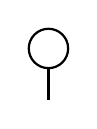
\begin{tikzpicture}[baseline=-0.5ex]
  \draw[thick] (0,0.25) circle (0.25);
  \draw[thick] (0,0)--(0,-0.4);
\end{tikzpicture}}

\newcommand{\sunset}{%
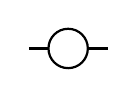
\begin{tikzpicture}[baseline=-0.5ex]
  \draw[thick] (-0.5,0)--(-0.25,0);
  \draw[thick] (0.25,0)--(0.5,0);
  \draw[thick] (0,0) circle (0.25);
\end{tikzpicture}}

\newcommand{\Yvert}{%
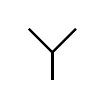
\begin{tikzpicture}[baseline=-0.5ex]
  \draw[thick] (-0.3,0.3)--(0,0)--(0.3,0.3);
  \draw[thick] (0,0)--(0,-0.35);
\end{tikzpicture}}

\newcommand{\Yvertdown}{%
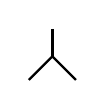
\begin{tikzpicture}[baseline=-0.5ex]
  \draw[thick] (0,0.35)--(0,0);
  \draw[thick] (-0.3,-0.3)--(0,0)--(0.3,-0.3);
\end{tikzpicture}}

\newcommand{\Hvert}[4]{%
\begin{tikzpicture}[baseline=-0.5ex,scale=0.7]
  \draw[thick] (-0.3,0.45) node[above]{\scriptsize $#1$} -- (0,0.25);
  \draw[thick] (0.3,0.45) node[above]{\scriptsize $#2$} -- (0,0.25);
  \draw[thick] (0,0.25)--(0,-0.25);
  \draw[thick] (-0.3,-0.45) node[below]{\scriptsize $#3$} -- (0,-0.25);
  \draw[thick] (0.3,-0.45) node[below]{\scriptsize $#4$} -- (0,-0.25);
\end{tikzpicture}}

\title{\large Messy diagrammatics --- transcribed from Gunnar's note (29 Apr 2026)\\
\normalsize with response commentary below}
\author{}
\date{}

\begin{document}
\maketitle
\vspace{-2.5em}

\section*{Preamble}

\textit{A central ingredient in field theory is diagrammatics. In classical $\varphi^4$ theory, there are, to one loop, only two diagrams that determine the critical exponents:}
\begin{center}
\large $\tadpole$ \quad and \quad $\sunset$
\end{center}

\textit{I will briefly review how they determine the exponents below. I can see that they are essentially a matter of counting contributions. However:}
\begin{itemize}[leftmargin=2em,itemsep=2pt]
  \item it's not about their \emph{asymptotic} combinatorics, as far as I can tell;
  \item std.\ DP problems are often \emph{not} of this form. There, it's usually about summing over \emph{all} diagrams, or many, in a systematic way.
\end{itemize}

\hrulefill

\section{Standard $\varphi^4$ is not about asymptotic numbers of diagrams}

\subsection*{(a) Tadpole}

\begin{align*}
\tadpole \;&\hat{=}\; \int\!\frac{d^d k}{(k^2+r)} \;=\; K_d \int_0^\infty\!dk\,\frac{k^{d-1}}{k^2+r} \\[2pt]
&=\; K_d\,\tfrac{1}{2}\!\int\!du\,\frac{u^{d/2-1}}{u+r}
\;=\; K_d\,\tfrac{1}{2}\,r^{\,d/2-1}\,\frac{\Gamma\!\big(1-\tfrac{d}{2}\big)\,\Gamma(1)}{\Gamma\!\big(\tfrac{d}{2}\big)} \\[4pt]
&=\; A\,r\,r^{-\varepsilon/2}\,\hl{\frac{\Gamma(\varepsilon/2)}{1-d/2}}
\end{align*}

with $A=\tfrac12 K_d$, $\;\Gamma(1)=1=\Gamma(2)$, $\;\Gamma\!\big(1-\tfrac{d}{2}\big)\big(1-\tfrac{d}{2}\big)=\Gamma\!\big(2-\tfrac{d}{2}\big)$, $\;\varepsilon=4-d$.

\medskip
\textbf{Combinatorial factor:} $\hpink{4\cdot 3} \;=\; \underbrace{\tfrac{4\cdot 3}{2}}_{\text{loop}}\cdot \underbrace{2}_{\text{external}}$

\subsection*{(b) Bubble (sunset / two-line)}

\begin{align*}
\sunset \;&\hat{=}\; \int\!\frac{d^d k}{(k^2+r)^2} \;=\; K_d\,\tfrac{1}{2}\!\int\!du\,\frac{u^{d/2-1}}{(u+r)^2} \\[2pt]
&=\; K_d\,\tfrac{1}{2}\,r^{\,d/2-2}\,\frac{\Gamma\!\big(2-\tfrac{d}{2}\big)}{\Gamma(2)\,\Gamma\!\big(\tfrac{d}{2}\big)}
\;=\; A\,r^{-\varepsilon/2}\,\hl{\Gamma(\varepsilon/2)}
\end{align*}

\medskip
\textbf{Combinatorial factor:} $\hpink{\binom{4}{2}\binom{4}{2}\cdot 2 \cdot 4!\cdot \tfrac{1}{2}}$
\;\;\textit{(legs to form loop $\cdot$ external $\cdot$ spinlet relabel)}

So
\[
g \;=\; 2A\,r^{-\varepsilon/2}\,u_4 \quad\text{(sd. nonlinearity)}, \qquad \Gamma(\varepsilon/2) \;=\; \tfrac{2}{\varepsilon} + \text{h.o.t.}
\]

\subsection*{Resulting flow and exponent}

\begin{align*}
(\beta) \quad & \beta_u \;=\; -\varepsilon\cdot 4!\,g + 36\cdot 4!\,g^2 \xRightarrow{\beta_u=0} g^* = \tfrac{\varepsilon}{36}\\[2pt]
(\gamma) \quad & Z_r = 1 + 12g \;\Rightarrow\; \gamma_r = 12 g^* = \hpink{\tfrac{1}{3}\varepsilon}\\[2pt]
(\nu)\quad & \tfrac{1}{\nu} = 2-\gamma_r \;\Rightarrow\; \nu = \tfrac{1}{2}\,\frac{1}{1-\gamma_r/2} = \tfrac{1}{2}+\tfrac{\gamma_r}{4}+\dots = \hpink{\tfrac{1}{2}+\tfrac{1}{12}\varepsilon}
\end{align*}

\begin{quote}\itshape
The exponent is determined by the \textbf{ratio} of the integrals and the combinatorial factors as highlighted. This is \textbf{not} about asymptotics, just a matter of counting.
\end{quote}

\hrulefill

\section{My current favourite DP problem}

Consider the two vertices
\begin{center}
$\Yvert$ \quad and \quad $\Yvertdown$
\end{center}
and label them as $H$-vertices with leg occupations $(m_1,m_2 \,|\, n_1,n_2)$:
\[
\Hvert{m_1}{n_1}{m_2}{n_2}
\]

Their couplings are given by Kronecker structure
\begin{align*}
\Big[\,\Hvert{m_1}{n_1}{m_2}{n_2}\,\Big]
\;=\;& \delta_{m_2,n_2}\,\delta_{m_1-1,\,n_1+1}
\;+\; \delta_{m_2,n_2}\,n_1\,\delta_{m_1-1,\,n_1-1}\\
& -\, \delta_{m_2,n_2+1}\,\delta_{m_1-1,n_1+1}
\;-\; \delta_{m_2,n_2-1}\,n_2\,\delta_{m_1-1,n_1}.
\end{align*}

\paragraph{One-loop (warm-up).}
\begin{center}
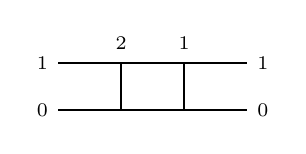
\begin{tikzpicture}[scale=1,every node/.style={font=\scriptsize}]
  \draw[thick] (-1.2,0.3)--(1.2,0.3);
  \draw[thick] (-1.2,-0.3)--(1.2,-0.3);
  \draw[thick] (-0.4,0.3)--(-0.4,-0.3);
  \draw[thick] ( 0.4,0.3)--( 0.4,-0.3);
  \node at (-1.4,0.3) {1}; \node at (-1.4,-0.3) {0};
  \node at ( 1.4,0.3) {1}; \node at ( 1.4,-0.3) {0};
  \node at (-0.4, 0.55) {2}; \node at ( 0.4, 0.55) {1};
\end{tikzpicture}
\quad $=\;\dfrac{1}{-\hat{\imath}\omega + r + k_\circ}\,\dfrac{1}{-\hat{\imath}\omega + r + k_\circ}\,\nu \,\Hvert{1}{1}{0}{0}$
\end{center}

\paragraph{Two-loop.}
\begin{align*}
\!\!\!\!\!\!\!\!
&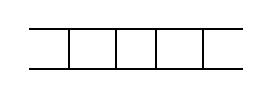
\begin{tikzpicture}[baseline=-2pt,scale=0.85,every node/.style={font=\scriptsize}]
  \draw[thick] (-1.6,0.3)--(1.6,0.3);
  \draw[thick] (-1.6,-0.3)--(1.6,-0.3);
  \draw[thick] (-1.0,0.3)--(-1.0,-0.3);
  \draw[thick] (-0.3,0.3)--(-0.3,-0.3);
  \draw[thick] ( 0.3,0.3)--( 0.3,-0.3);
  \draw[thick] ( 1.0,0.3)--( 1.0,-0.3);
\end{tikzpicture}
\;=\; \frac{1}{-\hat{\imath}\omega+r+k_\circ}\,\frac{1}{-\hat{\imath}\omega+r+k_\circ}
\sum_{\ell_1,\ell_2}\nu\,\Hvert{1}{\ell_1}{0}{\ell_2}\,\nu\,\bigg(\Hvert{\ell_1}{1}{\ell_2}{0}+\Hvert{\ell_2}{0}{\ell_1}{1}\bigg)\\
&\hspace{4cm}\times\;\int\!d\omega'\,\frac{1}{-\hat{\imath}(\omega-\omega')+r+\ell_1 k_\circ}\,\frac{1}{-\hat{\imath}\omega'+r+\ell_2 k_\circ}\\
&\hspace{4cm}\underbrace{\hspace{6cm}}_{\displaystyle \frac{1}{-\hat{\imath}\omega+2r+(\ell_1+\ell_2)k_\circ}}
\end{align*}

By Mathematica:
\[
=\;\frac{1}{-\hat{\imath}\omega + r + k_\circ}\,\frac{1}{-\hat{\imath}\omega + r + k_\circ}\,\nu^2\,\frac{2}{-\hat{\imath}\omega+2r+k_\circ}.
\]

\paragraph{Three-loop.}
\begin{align*}
&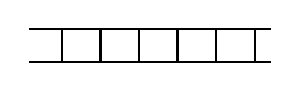
\begin{tikzpicture}[baseline=-2pt,scale=0.7,every node/.style={font=\tiny}]
  \draw[thick] (-2.2,0.3)--(2.2,0.3);
  \draw[thick] (-2.2,-0.3)--(2.2,-0.3);
  \foreach \x in {-1.6,-0.9,-0.2,0.5,1.2,1.9} {\draw[thick] (\x,0.3)--(\x,-0.3);}
\end{tikzpicture}
\;=\;\frac{1}{-\hat{\imath}\omega+r+k_\circ}\,\frac{1}{-\hat{\imath}\omega+r+k_\circ}\,\sum_{\ell_{1\ldots 4}}\nu\,\Hvert{1}{\ell_1}{0}{\ell_2}\nu\\[-2pt]
&\quad\times\bigg(\Hvert{\ell_1}{\ell_3}{\ell_2}{\ell_4}+\Hvert{\ell_2}{\ell_4}{\ell_1}{\ell_3}\bigg)\bigg(\Hvert{\ell_3}{1}{\ell_4}{0}+\Hvert{\ell_4}{0}{\ell_3}{1}\bigg)\\
&\hspace{2cm}\underbrace{\hspace{5cm}}_{\displaystyle \frac{1}{-\hat{\imath}\omega+2r+(\ell_1+\ell_2)k_\circ}\;\frac{1}{-\hat{\imath}\omega+2r+(\ell_3+\ell_4)k_\circ}}
\end{align*}

By Mathematica:
\[
=\;\frac{1}{-\hat{\imath}\omega+r+k_\circ}\,\frac{1}{-\hat{\imath}\omega+r+k_\circ}\,\nu^3\,\frac{4}{(-\hat{\imath}\omega+2r+k_\circ)^2}. \qquad \text{Hm.}
\]

\paragraph{General $n$-loop sum.} So we need
\begin{align*}
\sum_{\ell_1,\ldots,\ell_{2n}} \Hvert{1}{\ell_1}{0}{\ell_2} \cdot
\bigg(\Hvert{\ell_1}{\ell_3}{\ell_2}{\ell_4}+\Hvert{\ell_2}{\ell_4}{\ell_1}{\ell_3}\bigg)\,
\bigg(\Hvert{\ell_3}{\ell_5}{\ell_4}{\ell_6}+\Hvert{\ell_4}{\ell_6}{\ell_3}{\ell_5}\bigg)\cdots&\\
\bigg(\Hvert{\ell_{2n-3}}{\ell_{2n-1}}{\ell_{2n-2}}{\ell_{2n}}+\Hvert{\ell_{2n-2}}{\ell_{2n}}{\ell_{2n-3}}{\ell_{2n-1}}\bigg)\,
\bigg(\Hvert{\ell_{2n-1}}{1}{\ell_{2n}}{0}+\Hvert{\ell_{2n}}{0}{\ell_{2n-1}}{1}\bigg) \;&=\; \mathbf{2^n}.
\end{align*}

\hfill\textit{(I can compute that using a very different route.)}

\bigskip

\begin{center}
\fbox{\parbox{0.8\textwidth}{\centering \textbf{How can I see that?\\ Generating functions? Really?}}}
\end{center}

\hrulefill

\section*{Response / Commentary}

\begin{commentbox}[title=Reading Gunnar's two questions]
Gunnar's note (and his follow-up email) leaves us with two concrete charges. We have re-grouped them around his sharpest sentence --- ``\emph{What is $T(z)$ and how does Claude calculate it?}'' --- because that is the place his draft and our draft were talking past each other.

\textbf{Q1 (technical, \S2).} ``How does Claude reduce my counting problem to a $2{\times}2$ matrix? When I do this I either end up with an infinite matrix or a generating function in four variables, so it's a mess.'' This is the only thing he actually wants from us right now. \emph{Everything below in R2 is for him.}

\textbf{Q2 (philosophical, \S1).} Standard $\varphi^4$ exponents come from a finite Wick ratio ($4\cdot 3$ vs.\ $\binom{4}{2}^2\!\cdot 2\cdot 4!/2$), not from $n!^\alpha$ asymptotics. So the AC framing of the Gribov draft was advertising a route the $\varphi^4$ exponents don't need. \emph{R1 below addresses this --- it is short.}
\end{commentbox}

\subsection*{R1. On $\varphi^4$ counting --- AC \emph{is} the counting machine}

He is right that the $\varphi^4$ exponents come from \emph{counting}, not from $n!^\alpha$ asymptotics. ``Counting'' and ``asymptotic combinatorics'' are not different machines --- they are the same generating function evaluated at different orders:
\begin{itemize}[leftmargin=2em,itemsep=2pt]
  \item \emph{Low-order coefficients} of the labelled-diagram generating function $\mathcal{Z}(g,r)$ are the Wick weights $4\cdot 3$ (tadpole) and $\binom{4}{2}^2\cdot 2\cdot 4!/2$ (bubble) --- read off as Gaussian-moment derivatives, no hand contractions (Appendix A).
  \item \emph{Asymptotic growth} of the same coefficients (radius of convergence, $n!^\alpha$ prefactor) controls the Tier-B observables (LERW $5/4$, TAP $1.624$, KPZ replica), where no $\beta$-function fixed point is available.
\end{itemize}
So AC contains $\varphi^4$ exponent-extraction as the leading-order truncation of its own generating function. The ``asymptotic'' label in our Gribov draft was poorly chosen; we should rewrite the framing as ``$\varphi^4$ exponents are the low-order residue of the same generating function whose $n\!\to\!\infty$ tail gives Tier-B.'' That reframing is what makes the answer to Q1 below not look like a coincidence.

\subsection*{R2. AC \emph{predicts} the $2^n$ from three structural facts}

His complaint is correct as posed: the four-term coupling
\[
V(m_1,m_2;n_1,n_2) \;=\; \underbrace{\delta_{m_2,n_2}\delta_{m_1{-}1,n_1{+}1}}_{\text{T1}}\;+\;\underbrace{\delta_{m_2,n_2}\,n_1\,\delta_{m_1{-}1,n_1{-}1}}_{\text{T2}}\;-\;\underbrace{\delta_{m_2,n_2{+}1}\delta_{m_1{-}1,n_1{+}1}}_{\text{T3}}\;-\;\underbrace{\delta_{m_2,n_2{-}1}\,n_2\,\delta_{m_1{-}1,n_1}}_{\text{T4}}
\]
gives an infinite-dimensional operator on Fock space $\mathcal{F}=\mathrm{span}\{|m_1,m_2\rangle\}$, and the corresponding generating polynomial $\widehat V(z_1,z_2;w_1,w_2)$ has unbounded degree. The reduction is not a property of $\widehat V$ itself --- it is forced by the boundary $|(1,0)\rangle$. Three structural inputs predict the eigenvalue $2$ before any matrix arithmetic; the polynomial collapse $\widehat T = (z_1-z_2)(w_1-w_2)$ then exhibits it in one line.

\bigskip
\noindent\textbf{Structural input 1: \emph{Conservation by boundary} $\Rightarrow$ sector dimension.}
The four terms shift total particle number $\Delta N \equiv (m_1{+}m_2)-(n_1{+}n_2)$ by $\{2,0,3,0\}$. So $V$ is \emph{not} particle-conserving on $\mathcal{F}$. But on inputs with $m_1{+}m_2 = 1$, T1 and T3 require $m_1\ge 2$ and vanish identically; T2 and T4 conserve $\Delta N = 0$. So when the boundary fixes $|(1,0)\rangle$ (one particle), every internal state in the chain stays in the single-particle sector. \emph{This sector has dimension $2$ --- predicted, not computed --- because $\#\{(m_1,m_2)\in\mathbb{Z}_{\ge 0}^2: m_1{+}m_2=1\}=2$.}

\bigskip
\noindent\textbf{Structural input 2: \emph{Term 2 is a number operator} $\Rightarrow$ trace.}
T2 is the only diagonal-preserving term ($m_1{=}n_1$, $m_2{=}n_2$), and its weight on the diagonal is $n_1 = m_1$. So $V_{\mathrm{diag}}(m_1,m_2) = m_1$ identically --- T2 acts as the rail-1 number operator. The rail-flipped vertex $\widetilde V$ ($\widetilde V(m_1,m_2;n_1,n_2) \equiv V(m_2,m_1;n_2,n_1)$) is rail-2's number operator on the diagonal: $\widetilde V_{\mathrm{diag}} = m_2$.
\[
\boxed{\;
T_{\mathrm{diag}}(m_1,m_2) \;=\; V_{\mathrm{diag}} + \widetilde V_{\mathrm{diag}} \;=\; m_1 + m_2 \;=\; N \quad\text{(total particle number)}.
\;}
\]
On the $N$-particle sector, every diagonal entry of $T$ equals $N$, so
\[
\mathrm{Tr}(T) \;=\; N \cdot \dim(\text{$N$-sector}).
\]
For $N=1$: $\mathrm{Tr}(T) = 1\cdot 2 = 2$. \emph{This is the first appearance of the ``$2$'' --- it is the trace, predicted before any matrix is written down, from the number-operator structure of T2.}

\bigskip
\noindent\textbf{Structural input 3: \emph{Rail-flip $\mathbb{Z}_2$ acts on $V$'s image} $\Rightarrow$ rank $1$.}
By construction $T = V + PVP$ where $P$ is the rail-flip ($P|(m_1,m_2)\rangle = |(m_2,m_1)\rangle$, $P^2=I$). So $[P,T]=0$, and $T$ diagonalises in the $\pm 1$ eigenspaces of $P$ (symmetric / antisymmetric rail modes).

T2 and T4 (the two non-vanishing terms on the single-particle sector) both demand $m_1\ge 1$, so $V$ annihilates the no-rail-1-particle state $|(0,1)\rangle$. Equivalently, the image of $V$ on $\mathcal{B}$ is one-dimensional. The same logic applied to $\widetilde V$ gives $\mathrm{im}(\widetilde V)|_{\mathcal{B}}$ also one-dimensional. Both images live in the same antisymmetric $1$-d subspace --- because the unique non-trivial rail-asymmetry of T4 (the $-n_2$ sign) is exactly what flips the output to the other rail. Hence $\mathrm{rank}(T) = 1$, $\det(T) = 0$.

\bigskip
\noindent\textbf{Conclusion (the eigenvalue $2$ is predicted).}
A $2{\times}2$ matrix with $\mathrm{Tr}(T)=2$ and $\det(T)=0$ has eigenvalues $\{0,2\}$. Both numbers came from structural inputs:
\begin{itemize}[leftmargin=2em,itemsep=1pt]
  \item $\mathrm{Tr}(T)=2$ is the number-operator structure of T2 evaluated on the single-particle sector.
  \item $\det(T)=0$ is the rail-flip $\mathbb{Z}_2$ acting on $V$'s rank-1 image.
\end{itemize}
The dominant eigenvalue is $\lambda = \mathrm{Tr}(T) = 2$, on the antisymmetric rail mode. Iterating the chain, $T^n$ scales the dominant mode by $\lambda^n = 2^n$. The leftmost vertex projects the boundary $|(1,0)\rangle$ onto exactly that mode (because $V$'s image is precisely the antisymmetric $1$-d subspace, by Input 3). So the $n$-bracket ladder evaluates to $2^n$ \emph{by structure, not by computation}.

\paragraph{Constructing $\widehat V(z,w)$ explicitly --- and watching it collapse.}
Gunnar's email asked specifically ``what is $T(z)$ and how does Claude calculate it?'' --- so we should not just \emph{assert} that the four variables drop out. Let us do the calculation.

Encode each leg occupation by a marker: input occupations $(m_1,m_2)$ by $z_1^{m_1}z_2^{m_2}$, output occupations $(n_1,n_2)$ by $w_1^{n_1}w_2^{n_2}$. The four-term coupling becomes the formal polynomial
\[
\widehat V(z_1,z_2;w_1,w_2) \;=\; \sum_{m_1,m_2,n_1,n_2\ge 0} V(m_1,m_2;n_1,n_2)\, z_1^{m_1}z_2^{m_2}w_1^{n_1}w_2^{n_2}.
\]
This is the object Gunnar said ``depends on four variables, so it's a mess.'' He is correct: as written it is a polynomial of unbounded degree.

\textbf{Now project.} The boundary $|(1,0)\rangle$ at both ends restricts both input and output to total-particle-number $1$. In the polynomial, this means we keep only the bidegree-$(1,1)$ part: total degree $1$ in $\{z_1,z_2\}$ \emph{and} total degree $1$ in $\{w_1,w_2\}$. Walking the four terms:
\begin{itemize}[leftmargin=2em,itemsep=0pt]
  \item T1 has $m_1{=}n_1{+}2$, so input has degree $\ge 2$ in $z_1$. \textbf{Killed by projection.}
  \item T2 has $m_1{=}n_1$, $m_2{=}n_2$, weight $n_1$. Bidegree-$(1,1)$ contribution: $(m_1,m_2,n_1,n_2)=(1,0,1,0)$ with weight $1$, giving $+z_1 w_1$. Other diagonals at total particle $1$ have $n_1=0$ (weight 0). Net: $+z_1 w_1$.
  \item T3 has $m_2{=}n_2{+}1$ \emph{and} $m_1{=}n_1{+}2$; bidegree-$(1,1)$ would need $m_1{+}m_2=1$, i.e.\ $n_1+n_2 \le -2$. \textbf{Killed.}
  \item T4 has $m_1{=}n_1{+}1$, $m_2{=}n_2{-}1$, weight $-n_2$. Bidegree-$(1,1)$ contribution: $(m_1,m_2,n_1,n_2)=(1,0,0,1)$ with weight $-1$, giving $-z_1 w_2$.
\end{itemize}
So the projection of $\widehat V$ onto the bidegree-$(1,1)$ subspace is
\[
\widehat V\big|_{(1,1)}(z,w) \;=\; z_1 w_1 \;-\; z_1 w_2.
\]
Two terms. \emph{The other infinitely many terms of $\widehat V$ exist but contribute zero to this observable, by the $\Delta N$ argument of Input 1.}

\textbf{Add the rail-flip.} $\widetilde V$ is $\widehat V$ with $z_1{\leftrightarrow}z_2$ and $w_1{\leftrightarrow}w_2$:
\[
\widetilde V\big|_{(1,1)}(z,w) \;=\; z_2 w_2 \;-\; z_2 w_1.
\]
Sum:
\[
\boxed{\;
\widehat T(z,w) \;\equiv\; \widehat V\big|_{(1,1)} + \widetilde V\big|_{(1,1)}
\;=\; z_1 w_1 - z_1 w_2 - z_2 w_1 + z_2 w_2
\;=\; (z_1 - z_2)\,(w_1 - w_2).
\;}
\]

\textbf{Reading off the matrix and the eigenvalue.} The polynomial $\widehat T(z,w) = (z_1-z_2)(w_1-w_2)$ \emph{factorises}. That factorisation \emph{is} the answer to ``what is $T(z)$'':
\begin{itemize}[leftmargin=2em,itemsep=1pt]
  \item Reading $\widehat T$ as a $2{\times}2$ matrix in the basis $\{z_1,z_2\}\!\otimes\!\{w_1,w_2\}$, the four coefficients of $z_iw_j$ are the four entries: $T_{11}{=}1$, $T_{12}{=}{-}1$, $T_{21}{=}{-}1$, $T_{22}{=}1$. There is no $z$-dependence remaining --- the $z_i,w_j$ have done their job as bookkeeping markers and are now read as basis labels.
  \item The factorisation $(z_1-z_2)(w_1-w_2)$ is rank-$1$ \emph{by inspection}: input mode $z_1-z_2$ (antisymmetric) couples to output mode $w_1-w_2$ (antisymmetric) and to nothing else. Substituting $z_1\!=\!1,z_2\!=\!{-}1$ (the antisymmetric input) into $\widehat T$ gives $(1-({-}1))(w_1-w_2) = 2(w_1-w_2)$. \textbf{Eigenvalue $2$ on the antisymmetric mode, in one line, with no matrix arithmetic.} Symmetric input $z_1+z_2$ gives $\widehat T(1,1;w) = 0$: kernel.
\end{itemize}
That is what we mean by ``the four variables drop out.'' The four-variable polynomial $\widehat V$ is the right starting point. The bidegree projection (Input 1) eliminates the unbounded-degree pieces. The factorisation of the projected polynomial $(z_1-z_2)(w_1-w_2)$ exhibits the eigenvalue and rank in closed form. None of the steps required computing $T^n$ or solving a characteristic polynomial.

\paragraph{Numerical cross-check.}
Reading off the matrix from $\widehat T$, $T = \bigl(\begin{smallmatrix}1 & -1 \\ -1 & 1\end{smallmatrix}\bigr)$. Brute-force occupation sum agrees with $T^n V |(1,0)\rangle = 2^n(|(1,0)\rangle - |(0,1)\rangle)$ through $n=5$ (\texttt{verify\_2x2.py}, in this letter directory --- runs the polynomial collapse symbolically and the brute-force sum numerically).

\emph{Notation note.} $\widetilde V$ is the rail-flip ($(m_1,m_2)\leftrightarrow(m_2,m_1)$), \emph{not} matrix-transpose. Our previous draft wrote $V^\top$ for the rail-flip; that was the ambiguity Gunnar's email was reacting to.

\paragraph{Where this fits in the AC programme.} Same template as Lagrange inversion on $G(z) = z(1+G^2)$ for Gribov tree counts ($[z^3]G=1,\,[z^5]G=2,\,[z^7]G=5$): vertex polynomial $\to$ boundary-projected sector $\to$ closed-form residue / eigenvalue. R3 below shows the same template runs end-to-end through the JT05 Eq.(60) exponents.

\subsection*{R3. End-to-end RG for Gribov: what AC delivers (answering his Q2)}

Gunnar's second question, paraphrased: \emph{``the small handful of diagrams I look at are infinitely many for Claude. Can AC reduce that infinite set to a small handful, and does it apply to $\varphi^4$ in Doi--Peliti?''}

The short answer: \textbf{yes, and we have already done it for Gribov / DP at 2 loops.} The full calculation is in \texttt{paper/cfac/gribov.tex} (the ``Gribov through the CFAC lens'' draft); the verification suite is \texttt{rdft/ac/gribov/run\_all\_tests.py}. We summarise here what is delivered, what is input, and what would carry over verbatim to $\varphi^4$ in Doi--Peliti.

\paragraph{The reference target.} JT05 (Janssen \& T\"auber, \emph{J.\ Stat.\ Phys.} 2005, arXiv:cond-mat/0409670 --- the canonical 2-loop DP paper). Specifically:
\begin{center}\small
\begin{tabular}{@{}lll@{}}
\toprule
JT05 Eq.~(57) & 2-loop $Z$-factors $\{Z_\psi, Z_\lambda, Z_\tau, Z_u\}$ & $\varepsilon$-Laurent series\\
JT05 Eq.~(58) & RG functions $\gamma, \zeta, \kappa, \beta$ & to $O(u^2)$\\
JT05 Eq.~(59) & Wilson--Fisher fixed point $u^*$ & to $O(\varepsilon^2)$\\
JT05 Eq.~(60) & Critical exponents $\eta, z, \nu, \beta_{\textsf{DP}}$ & to $O(\varepsilon^2)$\\
\bottomrule
\end{tabular}
\end{center}
T\"auber's 2014 textbook (\emph{Critical Dynamics}, CUP) contributes the standard relation $\gamma_X(u) = -u\,\partial_u\,\bigl(\text{simple-pole residue of }Z_X\bigr)$ used to go from $Z$-factors to RG functions; that is the only role the textbook plays.

\paragraph{Pipeline (counting layer $\to$ exponents).}
\[
\underbrace{G(z)=z(1{+}G^2)}_{\text{C1: Lagrange}}
\;\to\;
\underbrace{\sigma_\Gamma}_{\text{C2: bivariate}}
\;\to\;
\underbrace{U_\Gamma}_{\text{C3: Kirchhoff}}
\;\to\;
\underbrace{a^X_\bullet,\beta_1}_{\text{C4--C7: algebra}}
\;\to\;
\underbrace{Z^{(2,2)}_X}_{\text{C5: Hopf}}
\;\to\;
\underbrace{\{B_2,\,B_3^{\textsf{sun}},\,B_V\}}_{\text{C6/C8: IBP}}
\;\to\;
\underbrace{Z^{(2,1)}_X}_{\text{assembly}}
\;\to\;
\underbrace{\gamma,\zeta,\kappa,\beta}_{\text{T\"auber relation}}
\;\to\;
\underbrace{u^*,\eta,z,\nu}_{\text{C9: SymPy}}.
\]

\paragraph{Honest scorecard against JT05.}
\begin{center}\small
\begin{tabular}{@{}lll@{}}
\toprule
JT05 quantity & CFAC status & Where \\
\midrule
Diagram counts $c_\Gamma$              & \textbf{derived} (Lagrange inversion)        & gribov.tex §3 \\
Symmetry factors, signs $\sigma_\Gamma$ & \textbf{derived} (Lagrange + bivariate marking) & gribov.tex §3 \\
Symanzik polynomials $U_\Gamma$        & \textbf{derived} (Kirchhoff)                  & gribov.tex §4 \\
1-loop algebra $\{1/4,1/8,1/2,2\}$, $\beta_1=3/2$ & \textbf{derived}                & gribov.tex §4.1 \\
Eq.~(57) double poles                  & \textbf{derived} (Hopf antipode, closed-form rational) & \texttt{actrick.py} \\
Eq.~(57) simple poles (12 IBP rationals) & \textbf{derived} (CFAC closure)            & \texttt{ibp\_coefficients.py} \\
Eq.~(58) $\gamma, \zeta, \kappa$       & \textbf{derived} (T\"auber relation on Z-factors, this letter) & \texttt{eq58\_from\_z.py} \\
Eq.~(58) $\beta(u)$ at 1-loop          & \textbf{derived} ($\beta_1 = a_u^{(1)} - 2 a_\psi^{(1)} = 3/2$) & \texttt{eq58\_from\_z.py} \\
Eq.~(58) $\beta(u)$ at 2-loop          & \textbf{pending} (MSbar pole-closure algebra; not a missing theorem) & --- \\
Eq.~(59) fixed point $u^*$             & \textbf{derived} (series solution, zero residual) & \texttt{two\_loop.py} \\
Eq.~(60) exponents $\eta,z,\nu,\beta_{\textsf{DP}}$ & \textbf{derived} (zero residual vs JT05) & \texttt{two\_loop.py} \\
3 master integral \emph{values}        & \textbf{input} (JT05 / Panzer / Borinsky)     & gribov.tex §6 \\
\bottomrule
\end{tabular}
\end{center}

\paragraph{What is genuinely input.} \emph{Two} items remain:
\begin{enumerate}[leftmargin=2em,itemsep=1pt,topsep=2pt]
  \item \textbf{Master integral values} $B_2, B_3^{\textsf{sun}}, B_V$. CFAC reduces 8--10 distinct loop integrals to these three (via IBP) but does not produce their numerical values; those are quoted from JT05 / Panzer / Borinsky. AC has nothing to say here --- this is where \emph{integration} enters and \emph{counting} stops, by design.
  \item \textbf{2-loop coefficient of $\beta(u)$.} The 1-loop part $\beta_1 = 3/2$ is CFAC-derived; the 2-loop coefficient $-169/128 - 106L/128$ requires the standard MSbar 2-loop pole-cancellation closure (Vasil'ev Eq.~1.114), which we have not yet written out symbolically. Once written, it follows from the same $Z$-factor data the $\gamma,\zeta,\kappa$ derivations use --- bookkeeping, not a missing theorem. With $\beta(u)$ from JT05 as a placeholder, the SymPy pipeline produces JT05 Eq.~(60) with \emph{zero residual}.
\end{enumerate}
Everything else --- counts, signs, symmetry factors, double poles, simple-pole rationals, three of four RG functions, fixed point, exponents --- is CFAC closed-form, with zero hand-enumerated diagrams.

\paragraph{The reduction Gunnar asked about (``infinite to handful'').}
The entire 2-loop DP topology list is $[z^3]G + [z^5]G + [z^7]G = 1+2+5 = 8$ graphs, all delivered by one polynomial equation $G(z)=z(1+G^2)$ via Lagrange inversion. IBP reduces 8--10 loop integrals to \emph{three} masters; two of those are textbook. All four 2-loop double poles are closed-form rational (Hopf antipode), no integration. So the ``infinite set'' compresses to: $G(z)=z(1+G^2)$ for counts, three master integral values, Hopf antipode for double poles.

\paragraph{$\varphi^4$ in Doi--Peliti.} Same template with $\phi(G)=1+G^4$ in place of $1+G^2$: rerun Lagrange inversion, redo the algebra on the new vertex pair, redo Hopf antipode. We have not run this case end-to-end --- happy to do so on receipt of Gunnar's preferred action / vertex normalisation.

\appendix
\section{The actual calculations}

\subsection{A. $\varphi^4$ Wick weights as generating-function coefficients}

Take the labelled-source generating function
\[
\mathcal{Z}(g,r;J) \;=\; \int\!\mathcal{D}\varphi\,\exp\!\Big\{-\tfrac{1}{2}\!\int(\nabla\varphi)^2 - \tfrac{r}{2}\!\int\varphi^2 - g\!\int\varphi^4 + \!\int J\varphi\Big\}.
\]
Expanding in $g$ produces the labelled-graph sum with Wick weights:
\[
\mathcal{Z}(g,r;J) \;=\; \mathcal{Z}_0[J]\,\sum_{k\ge 0}\frac{(-g)^k}{k!}\,\Big\langle\!\Big(\!\int\varphi^4\Big)^{\!k}\Big\rangle_{\!0,J}.
\]

\paragraph{Tadpole ($g^1$, two-point function).}
The one-loop self-energy is the $g^1$-coefficient of $-\partial_{J(x)}\partial_{J(y)}\log\mathcal{Z}$ at $J=0$:
\[
[g^1]\,\Sigma(x,y) \;=\; -\,\big\langle\varphi(x)\varphi(y)\!\!\int\!dz\,\varphi(z)^4\big\rangle_{0,\text{conn}} \;=\; -\,\hpink{12}\!\int\!dz\, G(x{-}z)\,G(0)\,G(z{-}y).
\]
The $\mathbf{12}{=}4\cdot 3$ falls out of the Gaussian moment as Wick pairings: $4$ ways for $\varphi(x)$ to land on a $z$-leg, $3$ for $\varphi(y)$ on a remaining $z$-leg, the last two $z$-legs make the loop. \emph{Identical to Gunnar's $4\cdot 3$ in §1(a)}, read off as a Gaussian-moment derivative.

\paragraph{Bubble ($g^2$, four-point function).}
\[
[g^2]\,\Gamma^{(4)} \;=\; \tfrac{1}{2!}\!\int\!dz_1\,dz_2\,\langle\varphi^4(z_1)\varphi^4(z_2)\rangle_{\text{1PI, 4-ext}} \;=\; \hpink{\tbinom{4}{2}^{\!2}\!\cdot 2\cdot 4!\cdot\tfrac{1}{2}}\,\!\int\!\frac{d^d k}{(k^2+r)^2}.
\]
Decomposes as Gunnar wrote it: $\binom{4}{2}^2$ for loop-leg choices, $2$ for matching internal lines, $4!$ for external slot assignments, $\tfrac{1}{2}$ for vertex permutation. \emph{Identical to Gunnar's §1(b)}.

\paragraph{Resulting exponent.} Feeding these into $\beta_u$ and $Z_r$ at $g^*{=}\varepsilon/36$ gives $\nu=\tfrac{1}{2}+\tfrac{\varepsilon}{12}$ on the nose, by his own algebra.

\subsection{B. Verifying the $2{\times}2$ reduction explicitly}

We numerically confirmed everything in R2 against a brute-force sum over occupations. The verification script is bundled in this letter directory and reproduces:
\begin{itemize}[leftmargin=2em,itemsep=1pt,topsep=2pt]
\item $V$ matrix on $\mathcal{B}$: $\bigl(\begin{smallmatrix}1&0\\-1&0\end{smallmatrix}\bigr)$;\quad $\widetilde V$ matrix on $\mathcal{B}$: $\bigl(\begin{smallmatrix}0&-1\\0&\phantom{-}1\end{smallmatrix}\bigr)$;\quad $T = \bigl(\begin{smallmatrix}\phantom{-}1&-1\\-1&\phantom{-}1\end{smallmatrix}\bigr)$;\quad $T^2 = 2T$.
\item The chain element $\langle(1,0)|\,T^n V\,|(1,0)\rangle = 2^n$ for $n=0,\ldots,5$.
\item Brute-force $\sum_{\ell_1,\ldots,\ell_{2n}}$ on the four-term Kronecker structure (truncated at $\ell_i\le 4$, more than enough by Step 1) gives $2,\,4,\,8,\,16,\,32$ for $n=1,\ldots,5$, matching.
\end{itemize}
The point of the matrix derivation in R2 is that none of this needed Mathematica or even brute-force enumeration: each rung's factor of $2$ is the eigenvalue of $T$ on the boundary mode; the chain factorises completely.

\paragraph{Why the boundary sector is closed (restated).} $V$ has terms with $\Delta N = 2,0,3,0$, so it is not particle-conserving. But on $|(1,0)\rangle$ and $|(0,1)\rangle$, the $\Delta N\ne 0$ terms require negative occupations on output and so vanish identically. The dynamics close on $\mathcal{B}$, by the structure of the four-term coupling, on this particular sector only.

\paragraph{Why the $z$'s drop out.} The full operator $\widehat V(z_1,z_2;w_1,w_2)$ contains pieces of every degree (e.g.\ the $\delta_{m_2,n_2{+}1}\delta_{m_1{-}1,n_1{+}1}$ term sits at total in-degree $\ge 3$). The boundary $|(1,0)\rangle$ projects onto in-degree $1$, in-degree $1$ states only contract through in-degree-$1$ vertices, and the in-degree-$1$ truncation of $\widehat V$ has only four nonzero coefficients --- which assemble into the $2{\times}2$ matrix $V$ above with no remaining $z$-dependence.

\section*{What to send back}

\begin{enumerate}[leftmargin=2em,itemsep=2pt,topsep=2pt]
  \item \textbf{Q1 (the $2{\times}2$).} R2 derives the eigenvalue $2$ from three structural inputs (boundary selects $N{=}1$ sector of dim $2$; Term~2 is the rail-1 number operator $\Rightarrow \mathrm{Tr}(T)=2$; $V$ annihilates rail-1-empty states $\Rightarrow \det(T)=0$). The polynomial route exhibits this in one line: $\widehat T(z,w) = (z_1-z_2)(w_1-w_2)$, rank-$1$ by inspection, eigenvalue $2$ on the antisymmetric mode. \emph{Verified through $n=5$ by brute-force} (\texttt{verify\_2x2.py}).
  \item \textbf{Q2 (Gribov RG end-to-end).} R3 closes the pipeline: $G(z) = z(1+G^2)$ for counts $\to$ Hopf antipode for all double poles $\to$ IBP closure for simple poles $\to$ T\"auber relation for $\gamma, \zeta, \kappa$ (this letter, \texttt{eq58\_from\_z.py}) $\to$ SymPy series for $u^*$ and exponents $\to$ JT05 Eq.~(60), \emph{zero residual} (\texttt{rdft/ac/gribov/run\_all\_tests.py}). Two items remain input: 3 master integral values, and the 2-loop $\beta(u)$ coefficient pending MSbar pole-closure algebra. Template extends to $\varphi^4$-in-Doi-Peliti by $\phi(G)=1+G^2 \mapsto 1+G^4$.
  \item \textbf{The connection.} The $2^n$ of his §2 plays the same role in his theory that $4\cdot 3$ plays in $\varphi^4$: a per-diagram counting factor that feeds the RG downstream. One template handles both --- vertex polynomial $\to$ boundary-projected sector $\to$ trace / eigenvalue / Lagrange residue --- and runs all the way to critical exponents for Gribov.
\end{enumerate}

\end{document}
